% easychair.tex,v 3.5 2017/03/15

\documentclass{easychair}
%\documentclass[EPiC]{easychair}
%\documentclass[EPiCempty]{easychair}
%\documentclass[debug]{easychair}
%\documentclass[verbose]{easychair}
%\documentclass[notimes]{easychair}
%\documentclass[withtimes]{easychair}
%\documentclass[a4paper]{easychair}
%\documentclass[letterpaper]{easychair}
\usepackage{wrapfig}
\usepackage{doc}
\usepackage{fullpage}
\usepackage{fancyvrb}
\usepackage{amsmath}
\usepackage{amssymb}

% use this if you have a long article and want to create an index
% \usepackage{makeidx}

% In order to save space or manage large tables or figures in a
% landcape-like text, you can use the rotating and pdflscape
% packages. Uncomment the desired from the below.
%
% \usepackage{rotating}
% \usepackage{pdflscape}

% Some of our commands for this guide.
%
\newcommand{\easychair}{\textsf{easychair}}
\newcommand{\miktex}{MiK{\TeX}}
\newcommand{\texniccenter}{{\TeX}nicCenter}
\newcommand{\makefile}{\texttt{Makefile}}
\newcommand{\latexeditor}{LEd}
\def\MC{{\sf MC}}
\def\HB{{\sf HB}}
\def\newterm#1{{\it #1}}

%\makeindex

%% Front Matter
%%
% Regular title as in the article class.
%
\title{Porting the Mathematical Components library to Hierarchy Builder}

% Authors are joined by \and. Their affiliations are given by \inst, which indexes
% into the list defined using \institute
%
\author{
  Reynald Affeldt\inst{3}
  \and
  Xavier Allamigeon\inst{4}
  \and
  Yves Bertot\inst{1}
  \and
  Quentin Canu\inst{4}
  \and
  Cyril Cohen\inst{1}
  \and
  %Marie Kerjean
  %\and
  Pierre Roux\inst{6}
  \and
  Kazuhiko Sakaguchi\inst{2}
  \and
  Enrico Tassi\inst{1}
  \and
  Laurent Th\'ery\inst{1}
  \and
  Anton Trunov\inst{5}
}

% Institutes for affiliations are also joined by \and,
\institute{
  Universit\'e C\^ote d'Azur, Inria, France
\and
   University of Tsukuba, Japan
\and
   National Institute of Advanced Industrial Science and Technology (AIST), Japan
\and
   Inria, CMAP, CNRS, Ecole Polytechnique, Institut Polytechnique de Paris, France
\and
   Zilliqa Research
\and
 ONERA / DTIS, Universit\'e de Toulouse, France
}

%  \authorrunning{} has to be set for the shorter version of the authors' names;
% otherwise a warning will be rendered in the running heads. When processed by
% EasyChair, this command is mandatory: a document without \authorrunning
% will be rejected by EasyChair

\authorrunning{The Mathematical Components developers}

% \titlerunning{} has to be set to either the main title or its shorter
% version for the running heads. When processed by
% EasyChair, this command is mandatory: a document without \titlerunning
% will be rejected by EasyChair
\titlerunning{Mathematical Components and Hierarchy Builder}

\begin{document}

\maketitle

% The table of contents below is added for your convenience. Please do not use
% the table of contents if you are preparing your paper for publication in the
% EPiC Series or Kalpa Publications series

%\setcounter{tocdepth}{2}
%{\small
%\tableofcontents}

%\subsection*{To mention}
%
%Processing in EasyChair - number of pages.
%
%Examples of how EasyChair processes papers. Caveats (replacement of EC
%class, errors).

%------------------------------------------------------------------------------
%\subsection*{Context}
%\label{sect:introduction}
~\\
We report on the porting of the Mathematical Components library (hereafter \MC{})
to the Hierarchy Builder~\cite{cohen_et_al:LIPIcs:2020:12356} tool (hereafter \HB{}).

\MC{} is an extensive and coherent repository of formalized
mathematical theories. At the time of writing about 40 opam packages depend
on some components from this library and these packages are not exclusively
focusing on mathematics (e.g., QuickChick, Disel, \ldots). To our
knowledge about 100 papers about formal proofs build on top of \MC{}.
The library is made of 91 files for a total 124 000 lines of code.

The key to keep the library growing in a rational way is that it revolves
around a hierarchy of interfaces which organizes operations and properties.
Interfaces come with theories which apply, automatically, to all the objects
which are registered as validating the interface. These interfaces are
implemented following the packed classes discipline which works well in practice
but has never been easy to master. Pull Requests extending or modifying the
hierarchy turned out to be problematic, hard to review and integrate due to their
length and complexity. Only
a few were merged, the others were put on hold waiting for the library to be
ported to \HB{}.

\begin{wrapfigure}[16]{r}{.35\textwidth}
  \vspace{-1em}
	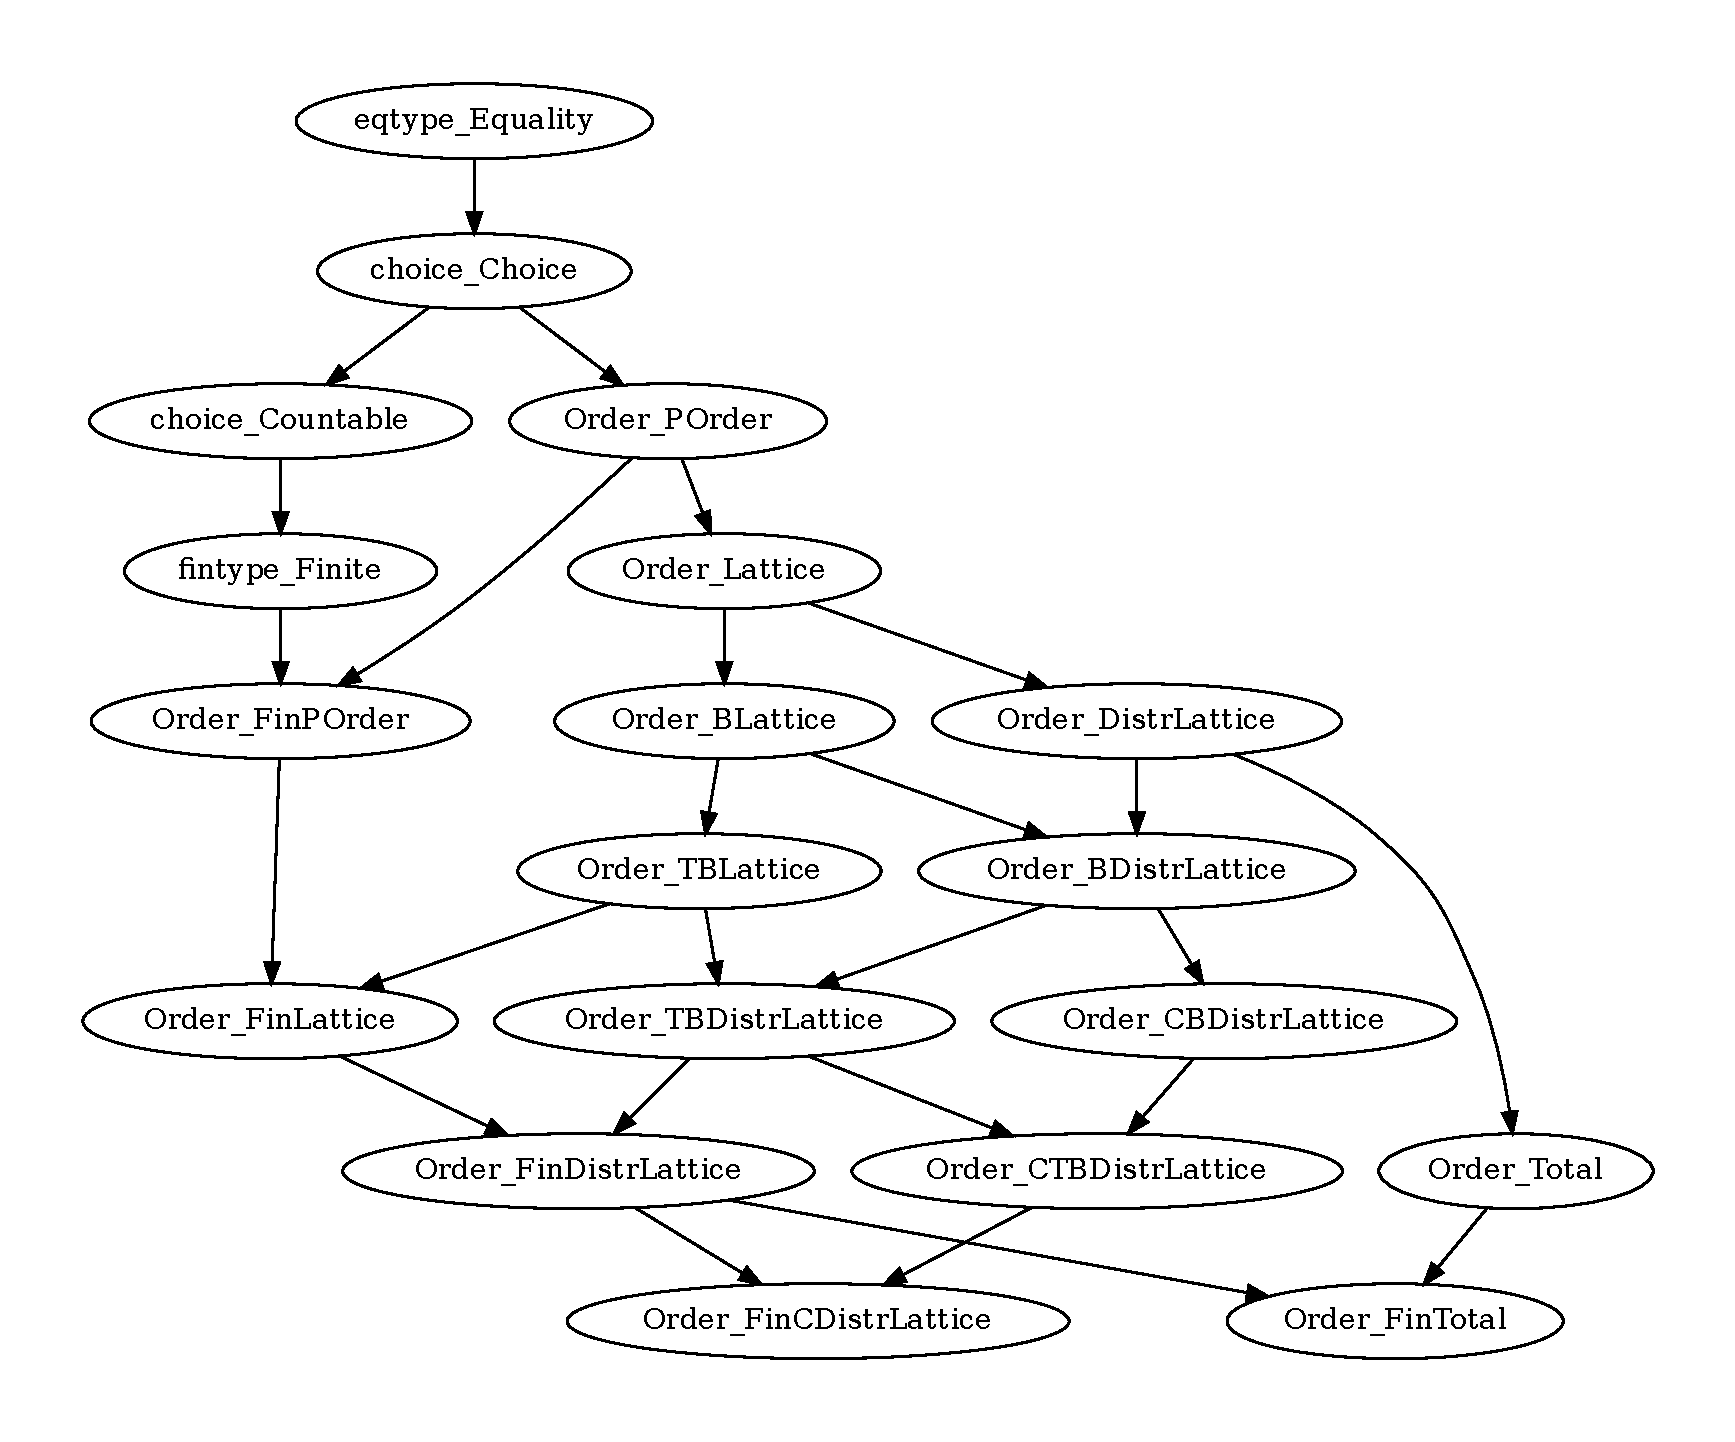
\includegraphics[width=.35\textwidth]{order.pdf}
  \caption{\small Hierarchy in {\tt order.v}}
	\label{fig:order}

\end{wrapfigure}
\
\HB{} is a set of high level vernacular commands implemented in Coq-Elpi, an
extension language for Coq developed by Tassi. \HB{} takes
care of automatically synthesizing all the error prone boilerplate required for
packed classes to work. Users just input record declarations,
standing for the interfaces, and proofs, for the instances.
They are relieved from
most of the gibberish of modules, sections, coercions, canonical
structures, implicit arguments, phantom abbreviations, \ldots

In the week from the 6th to the 9th of April 2021 the authors of this abstract
gathered (virtually) for a sprint on porting the \MC{} library to
\HB{}. The whole library finally compiled on April 20.
The porting consisted of declaring all the interfaces and their instances
using the new commands, \emph{without changing proofs} in any substantial way.
At the time of writing the patch (\href{https://github.com/math-comp/math-comp/pull/733}{math-comp\#733})
amounts to about 5K lines being edited (the declaration of the hierarchy and
the declarations of canonical instances), and 5K lines being simply \emph{removed}.\\
\
%\vspace{-2em}
%\subsection*{Report}
\paragraph{Documentation}
\HB{} is a young tool lacking documentation
on how to use it proficiently. Some of this knowledge emerged
during the sprint and is being archived in the wiki of the project
% (\href{https://github.com/math-comp/math-comp/wiki/HB-porting}{HB-porting})
and we plan to share it with the Coq community at the workshop.

The documentation of the \MC{} library itself is also being reworked, updating
the file headers with the new interfaces the user is supposed to use.
In order to ease the documentation effort we extended \HB{} with two commands,
one to draw the hierarchy of interfaces, see Figure~\ref{fig:order} for the excerpt
for the order component, and another one similar to \verb+About+ to access
metadata specific to the hierarchy, like the known instances of an interface
and where they are declared.
% Thanks to the fact that \HB{} has an internal representation of the hierarchy we could provide a command to
% generate a dot presentation of it, see~\ref{fig:order} for the excerpt for the
% order component, which lost 1300 lines in the process. In addition to that about command to get \HB{}
% specific info.
%
% \begin{wrapfigure}[12]{r}{.40\textwidth}
% \vspace{-1em}
% \begin{Verbatim}[fontsize=\footnotesize]
%  HB: Order.Total.type is a structure
%      (from "./ssreflect/order.v", line 1588)
%  HB: Order.Total.type characterizing operations
%      and axioms are:
%      - le_total
%  ...
%  HB: Order.Total inherits from:
%      - eqtype.Equality
%      - choice.Choice
%      - Order.POrder
%      - Order.Lattice
%      - Order.DistrLattice
%  HB: Order.Total is inherited by:
%      - Order.FinTotal
% \end{Verbatim}
% \vspace{-1.5em}
% \caption{\small {\tt HB.about.}}
% \label{fig:orderabout}
% \end{wrapfigure}
%
\paragraph{Performance}

When definitions pile up, unfolding
them can lead to terms which are too large to handle even for a computer,
and Type Theory provides no lightweight way to enforce abstraction barriers.
In order to prevent performance issues the \MC{} library ``locks''
some definitions, hiding them behind module signatures.
Since \HB{} uses a less ``efficient'' representation of
structures (more regular, not hand-optimized) we had to lock a handful
more definitions.
Given that the \MC{} library was already built with abstraction barriers
in mind --
once a new concept is defined and all its theory is proved, the client
is never supposed to unfold the concept -- the changes needed to adapt
proofs (unlocking concepts) were minimal. We extended \HB{} with
a lock command which takes care of the rather verbose declarations of modules
and their signatures.

\paragraph{Lightweight factories}

\HB{} provides a built-in concept of \newterm{factory}, a virtual interface which is
compiled to real interfaces automatically. % They are mandatory to get backward
%compatibility when a library evolves.
However, sometimes, defining a factory is
unnecessarily heavy and we prefer to rely on either one or a combination of the
following techniques: we use a lemma which produces a
factory from some (smaller) input; we declare a type alias (identity definition)
which already validates some interfaces and we copy all its instances to a new
type via an automatically generated tool. For example
\verb+Countable.copy T (can_type fgK)+ equips a type \verb+T+ with
\verb+Countable+, \verb+Choice+ and \verb+Equality+ instances proviso a
proof \verb+(fgK : cancel f g)+ where \verb+cancel f g+ expresses the fact
that \verb+(f : T -> T')+ and \verb+g+ are inverse functions, and where \verb+T'+
is already a \verb+Countable+ type.

\paragraph{Limitations}

\MC{} defined a normed $\mathbb{Z}$-module as a
$\mathbb{Z}$-module equipped with a norm with values in a numeric domain,
and a numeric domain as a $\mathbb{Z}$-module on itself; this apparent
cyclicity which was encodable by hand~\cite{affeldt:hal-02463336}
is not supported by \HB{}.
Since these structures are only really needed in \MC{}-analysis,
we managed to port \MC{} by oversimplifying them.
We plan to extend \HB{} to support this kind of self-reference
thus enabling the porting of \MC{}-analysis. There are also hierarchies of
morphisms and subobjects in \MC{}, while we could have ported the former,
the latter follows a design pattern that is not yet
supported by \HB{}.

\paragraph{The coding sprint}

One of the challenges of the sprint was to contribute simultaneously
to several \MC{} files and eventually update \HB{} with fixes for blocking bugs.
We used a locking mechanism based on Github's check list on the pull request,
whose advancement status was also reflected on the file graph of the library.
Moreover we systematically used a Zulip stream and a Jitsi video chat per file,
allowing the developers to work in small groups,
share their knowledge and progress and quickly reach out for help. Using Nix to describe the development
environment helped keeping the continuous integration in sync with the
environment used by the developers.
Still, we could have benefited from more tool support. In particular,
an UI that would allow executing in parallel two versions of a Coq script
would have been a plus in this porting activity.

\paragraph{Impact on \MC{} users and perspectives}

The switch to \HB{} will lead to \MC{} version 2.0. Updating to it will cause
breakage but we believe the benefits outweigh the porting burden,
if only because we will then be able to rework the hierarchy
\emph{without breaking client code}, since factories can serve as backward
compatible interfaces. Moreover it will trigger a number
of immediate improvements to the library from the addition of new, long awaited,
structures like semilattices and semirings to the integration of existing user
developments (e.g., dioid).
%
Still, since \MC{} is widely used, we plan to continue
maintaining the 1.x branch even after version 2.0 is released
(possibly backporting updates which don't require changing the hierarchy).

\label{sect:bib}
\bibliographystyle{plain}
%\bibliographystyle{alpha}
%\bibliographystyle{unsrt}
%\bibliographystyle{abbrv}
\bibliography{bib}

%------------------------------------------------------------------------------


\end{document}

